%!TeX program = lualatex
\documentclass[titlepage]{article}
\usepackage{../Head}
\usepackage{relsize}
\graphicspath{.}
\begin{document}
\fancyhf{}
\fancyhead[RO,R]{Advanced Calculus 420}
\fancyhead[LO,L]{Dakota Wicker}
\fancyhead[CO,C]{Homework VI}
\cfoot{\thepage}
\begin{cproblem}{1}{White}
Consider the following torus obtained by revolving a circle of radius $b$ around a circle of radius $a$, where $a\leq b$. 
\begin{center}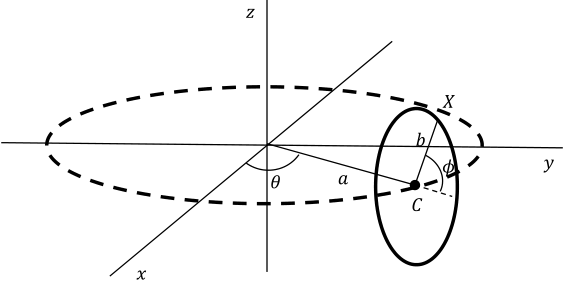
\includegraphics[scale=.6]{torus}\end{center}\phantom{.}
\vspace{-2em}
\begin{itemize}
\item[a.] Use the fact that $\vec{X} = \vec{C} + \vec{CX}$ to derive the following paramatric equations of the torus.
\begin{align*}
x = a\cos(\theta) &+ b\cos(\phi)\cos(\theta) \\ 
y = a\sin(\theta) &+ b \cos(\phi)\sin(\theta) \\
z =&\ b\sin(\phi) \\
0\leq \phi \leq 2\pi&, \quad 0\leq\theta\leq 2\pi
\end{align*}
\vspace{-2em}
\item[b.] Use this parameterization to find the surface area of the torus.
\end{itemize}
\end{cproblem}
\begin{solution}
\vspace{-2em}
\begin{itemize}
\item[a.]
Using basic trigonometry properties and the diagram above, I get that the $x$ component of $\vec{C}$ is just $a\cos(\theta)$, the $y$ component is just $a\sin(\theta)$ and the $z$ component is zero. This is from the triangle that $\vec{C}$ makes with the $x$ axis. Next I get that the $z$ component of $\vec{CX}$ is $b\sin(\phi)$ and by using the diagram by projecting $\vec{X}$ onto the $x,y$ plane, I get that the $y$ component of $\vec{CX}$ is  $b\cos(\phi)\sin(\theta)$ and finally, the $x$ component to be $b\cos(\phi)\cos(\theta)$.
So, it follows that
\begin{align*}
&\vec{X} = \vec{C} + \vec{CX} = \bmat{a\cos(\theta) \\ a\sin(\theta) \\ 0} + \bmat{b\cos(\phi)\cos(\theta) \\ b\cos(\phi)\sin(\theta) \\ b\sin(\phi)} = \bmat{a\cos(\theta) + b\cos(\phi)\cos(\theta) \\  a\sin(\theta) + b\cos(\phi)\sin(\theta) \\   b\sin(\phi)} \\
&\implies x = a\cos(\theta) + b\cos(\phi)\cos(\theta), \ y = a\sin(\theta) + b \cos(\phi)\sin(\theta), \ z = b\sin(\phi).
\end{align*}
\item[b.] It is known that the surface area over a surface $\Sigma$ is
$$\bigiint{\Sigma}{}dS = \bigiint{R}{}\sqrt{\left(\frac{\p(y,z)}{\p(\phi,\theta)}\right)^2 + {\left(\frac{\p(z,x)}{\p(\phi,\theta)}\right)}^2 +  \left(\frac{\p(x,y)}{\p(\phi,\theta)}\right)^2} \,d\phi\,d\theta$$
given a transformation $(x,y,z) \rightarrow (\phi,\theta)$ which maps $\Sigma$ to $R$.
So,
\begin{align*}
\frac{\p(y,z)}{\p(\phi,\theta)} &= \bigg|\bmat{ -b\sin(\phi)\cos(\theta) & a\cos(\theta) + b\cos(\phi)\cos(\theta) \\ b\cos(\phi) & 0 }\bigg|\\
\frac{\p(z,x)}{\p(\phi,\theta)} &= \bigg|\bmat{b\cos(\phi) & 0 \\ -b\sin(\phi)\cos(\theta) & -a\sin(\theta) - b\cos(\phi)\sin(\theta) }\bigg| \implies \bigiint{\Sigma}{}dS = \bigiint{R}{}ab+b^2\cos(\phi)\,d\phi\,d\theta. \\
\frac{\p(x,y)}{\p(\phi,\theta)} &= \bigg|\bmat{ -b\sin(\phi)\cos(\theta) & -a\sin(\theta) - b\cos(\phi)\sin(\theta)  \\ -b\sin(\phi)\sin(\theta) & \phantom{-}a\cos(\theta) + b\cos(\phi)\cos(\theta)}\bigg|
\end{align*}
Since $0\leq \phi \leq 2\pi, \ 0\leq\theta\leq 2\pi$, the surface area of the torus is
$$\mlvarint\limits_{0}^{2\pi} \left[\mlvarint\limits_{0}^{2\pi} ab+b^2\cos(\phi)\,d\phi\right]d\theta = 4\pi^2ab.$$
\end{itemize}
\end{solution}

\begin{cproblem}{2}{White}
\phantom{-}\\
\vspace{-1em}
\begin{itemize}
\item[a.]
Show that if a surface is described by $\Sigma = \{(x,y,z)\ | \ z= z(x,y), \ (x,y) \in R\}$, then the surface area is given by
$$S  = \bigiint{\Sigma}{}dS = \bigiint{R}{}\sqrt{1+\left(\frac{\p z}{\p x}\right)^2 + \left(\frac{\p z}{\p y}\right)^2}dxdy$$
\item[b.]Find the area of the surface
$$z = x^\frac{3}{2} + y^\frac{3}{2}$$
located above the square $0 \leq x, \ y\leq 1.$
\end{itemize}
\end{cproblem}
\begin{solution}
\begin{itemize}
\vspace{-2em}
\item[a.] \phantom{-} \\
It is known that $S = \bigiint{\Sigma}{}dS = \bigiint{R}{}\sqrt{\left(\frac{\p (y,z)}{\p(x,y)}\right)^2 + \left(\frac{\p (z,x)}{\p (x,y)}\right)^2 + \left(\frac{\p (x,y)}{\p (x,y)}\right)^2}\,dx\,dy$. \\Given that $\Sigma = \{(x,y,z)\ | \ z= z(x,y), \ (x,y) \in R\}$ I can parameterize the surface by this transformation. 
\begin{align*}
x &= x \\
y &= y \\
z &= z(x,y)
\end{align*}
This allows me to compute the corresponding jacobians.
\begin{align*}
\frac{\p(y,z)}{\p(x,y)} &= \bigg|\bmat{0 & 1 \\ \frac{\p z}{\p x} & \frac{\p z}{\p y}} \bigg| = -\frac{\p z}{\p x}\\
\frac{\p(z,x)}{\p(x,y)} &= \bigg|\bmat{\frac{\p z}{\p x} & \frac{\p z}{\p y} \\ 1 & 0} \bigg| = -\frac{\p z}{\p y}\\ 
\frac{\p(x,y)}{\p(x,y)} &= \bigg|\bmat{1 & 0 \\ 0 & 1} \bigg| = 1\\
\end{align*}
So by substitution, the surface area is
$$S = \bigiint{\Sigma}{}dS = \bigiint{R}{}\sqrt{\left( -\frac{\p z}{\p x}\right)^2 + \left(-\frac{\p z}{\p y}\right)^2 + 1^2}\,dx\,dy = \bigiint{R}{}\sqrt{1+\left(\frac{\p z}{\p x}\right)^2 + \left(\frac{\p z}{\p y}\right)^2}\,dx\,dy$$
\item[b.] \phantom{-} \\
Since this surface is described by $\Sigma = \{(x,y,z) \ | \ z(x,y), \ (x,y) \in R\}$, where $R = \{(x,y) \ | \ 0 \leq x,y \leq 1\}$ the surface area can be described as
$$ \bigiint{R}{}\sqrt{1+\left(\frac{\p z}{\p x}\right)^2 + \left(\frac{\p z}{\p y}\right)^2}\, dx\,dy. = \mlvarint\limits_{0}^{1} \left[\mlvarint\limits_{0}^{1}\sqrt{1+\left(\frac{\p z}{\p x}\right)^2 + \left(\frac{\p z}{\p y}\right)^2}\, dx \right]dy$$
and it is true that
\begin{align*}
\frac{\p z}{\p x} &= \frac{3}{2}x^{\frac{1}{2}} \\
\frac{\p z}{\p y} & = \frac{3}{2}y^{\frac{1}{2}}
\end{align*}
So by substitution the surface area is equal to
$$ \mlvarint\limits_{0}^{1} \left[\mlvarint\limits_{0}^{1}\sqrt{ \left(\frac{3}{2}x^{\frac{1}{2}}\right)^2 + \left(\frac{3}{2}y^{\frac{1}{2}}\right)^2 + 1}\, dx \right]dy = \mlvarint\limits_{0}^{1} \left[\mlvarint\limits_{0}^{1}\sqrt{ \frac{9x}{4} + \frac{9y}{4} + 1}\, dx \right]dy = \frac{968\sqrt{22} - 676\sqrt{13} + 64}{1215}.$$
\end{itemize}
\end{solution}

\begin{cproblem}{3}{White}
\phantom{-}
\begin{itemize}
\item[a.] 
Show that the unit sphere can be parameterized by 
$$ x = \sin(\phi)\cos(\theta), \quad y = \sin(\phi)\cos(\theta), \quad z = \cos(\phi)$$
$$ 0\leq\phi\leq \pi, \quad 0\leq\theta\leq 2\pi $$
\item[b.]
Find the flux of the vector field $\vec{A} = \smat{x \\ y \\ z}$ through the unit sphere oriented so that its orientation matches that of the $\phi, \theta$ plane.
\end{itemize}
\end{cproblem}
\begin{solution}\begin{center}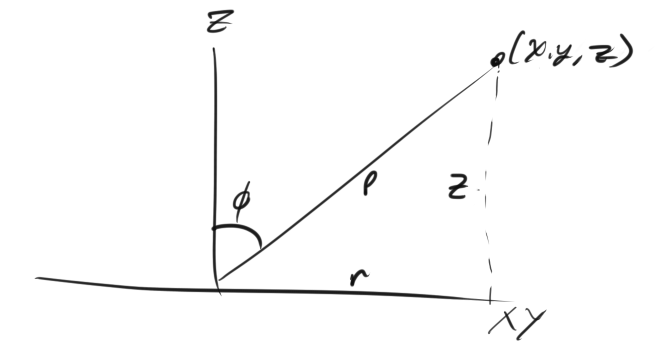
\includegraphics[scale=.5]{sphere.png}\end{center}
\begin{itemize}
\item[a.] The diagram above shows a point on the sphere in $x,y,z$ space with radius $\rho$. Using the diagram and trigonometry properties I see that the following is true
\begin{align*}
z &= \rho\cos(\phi) \\
r &= \rho\sin(\phi) 
\end{align*}
I can also describe the $(x,y,z)$ coordinate by using cylindrical coordinates. That is,
\begin{align*}
x &= r\cos(\theta) \\
y &= r\sin(\theta) \\
z &= z.
\end{align*}
Now, by substitution it is true that the parameterization of the (unit $\rho = 1$) sphere  is
\begin{align*}
x &= \rho\sin(\phi)\cos(\theta) \phantom{\implies} \ x  = \sin(\phi)\cos(\theta)\\
y &= \rho\sin(\phi)\sin(\theta) \overset{\rho = 1}{\implies} y = \sin(\phi)\sin(\theta) \\
z &= \rho\cos(\phi)\phantom{\cos(\theta) \implies} z =\cos(\phi).
\end{align*}
\item[b.] 
Given some transformation from $(x,y,z)$ to $(\phi,\theta)$ I know that flux is described by
$$ \bigiint{R}{} A_1\frac{\p (y,z)}{\p (\phi,\theta)} + A_2 \frac{\p (z,x)}{\p (\phi,\theta)} + A_3 \frac{\p (x,y)}{\p (\phi,\theta)}\,d\phi\,d\theta$$
where $\vec{A} = \smat{A_1 \\ A_2 \\ A_3}$, $R$ is the region that describes the unit sphere, and that
\begin{align*}
\frac{\p (y,z)}{\p (\phi,\theta)} &= \bigg|\bmat{\cos(\phi)\sin(\theta) & \phantom{-}\sin(\phi)\cos(\theta) \\ -\sin(\phi) & 0}\bigg| = \sin^2(\phi)\cos(\theta) \\
\frac{\p (z,x)}{\p (\phi,\theta)} &= \bigg|\bmat{-\sin(\phi) & 0 \\ \cos(\phi)\cos(\theta) & -\sin(\phi)\sin(\theta)}\bigg| = \sin^2(\phi)\sin(\theta) \\
\frac{\p (x,y)}{\p (\phi,\theta)} &= \bigg|\bmat{\cos(\phi)\cos(\theta) & -\sin(\phi)\cos(\theta) \\ \cos(\phi)\sin(\theta) & \phantom{-}\sin(\phi)\cos(\theta)}\bigg| = \sin(\phi)\cos(\phi ) 
\end{align*}
By subtitution the flux become as simple as 
$$\bigiint{R}{} \sin(\phi)\,d\phi\,d\theta$$
But I first need to describe $R$. I look at the unit sphere in $(x,y,z)$ space, $\Sigma = \{(x,y,z) \ | \ x^2 + y^2 + z^2 = 1, \ x,y,z \in \R^+\}$, what I want to do is to transform this into $(\phi,\theta)$ space. To do this I insert a diagram below
\begin{center}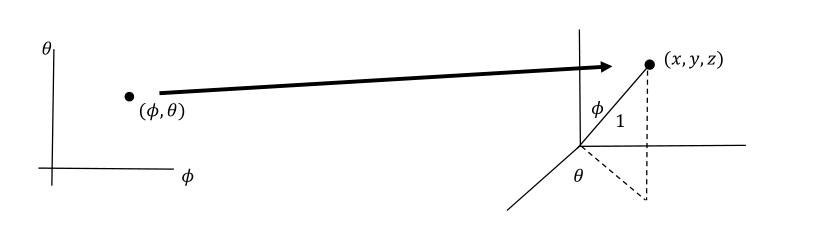
\includegraphics[scale=.7]{transform.png} \end{center}
and I notice that in $(x,y,z)$ space $\phi$ and $\theta$ are constricted by $x^2 + y^2 + z^2 = 1$ and only have the freedom of $0\leq\theta\leq2\pi, \ 0\leq\phi\leq\pi$. So, in the $(\phi,\theta)$ space the coordinate $(\phi,\theta)$ can only move around the rectangle bounded by $\theta = 2\pi, \ \theta = 0$ and $\phi = \pi, \ \phi = 0$. So, it follows that
$$R = \{(\phi,\theta) \ | \ 0\leq\phi\leq\pi , \ 0\leq\theta\leq2\pi\} $$
So, the flux of the field $A$ through the field through the unit sphere is
$$\mlvarint\limits_{0}^{2\pi}\left[\mlvarint\limits_{0}^{\pi} \sin(\phi)\,d\phi\right]d\theta = 4\pi.$$
\end{itemize}
\end{solution}
\clearpage
\begin{cproblem}{4}{White}\vspace{-.5em}
Suppose we have a fluid flowing with a velocity vector $\vec{A} = \smat{y^2 \\ 2z \\ -1}$. Find the flux of this fluid through the paraboloid $z = x^2 + y^2, \ 0 \leq x^2 + y^2 \leq 1$, where the orientation matches our usual orientation in the $x,y$ plane.
\end{cproblem}
\begin{solution}
Consider the transformation \\
\begin{align*}
x &= r\cos(\theta) \\
y &= r\sin(\theta) \\
z &= z.
\end{align*}
It follows that $z = x^2 + y^2 = r^2, \ \vec{A} = \smat{r^2\sin^2(\theta) \\ 2r^2 \\ -1}$, and, $0\leq r^2 \leq 1.$ Using this information it follows that the surface $\Sigma = \{(x,y,z) \ | \ z = x^2 + y^2, \ 0\leq z \leq 1, \ x,y \in \R\}$ becomes $R = \{(r,\theta) \ | \ 0\leq r \leq 1, \ 0\leq \theta \leq 2\pi\}$. So the flux of the vector field $\vec{A}$ through this surface is
$$ \bigiint{R}{} A_1\frac{\p (y,z)}{\p (r,\theta)} + A_2 \frac{\p (z,x)}{\p (r,\theta)} + A_3 \frac{\p (x,y)}{\p (r,\theta)}\,dr \,d\theta$$
and since $R = \{(r,\theta) \ | \ 0\leq r \leq 1, \ 0\leq \theta \leq 2\pi\}$ and 
\begin{align*}
\frac{\p (y,z)}{\p (\phi,\theta)} &= \bigg|\bmat{\sin(\theta) & r\cos(\theta) \\ 2r & 0}\bigg| = -2r^2\cos(\theta) \\
\frac{\p (z,x)}{\p (\phi,\theta)} &= \bigg|\bmat{2r & 0 \\ \cos(\theta) & -r\sin(\theta)}\bigg| = -2r^2\sin(\theta) \\
\frac{\p (x,y)}{\p (\phi,\theta)} &= \bigg|\bmat{\cos(\theta) & -r\sin(\theta) \\ \sin(\theta) & r\cos(\theta)}\bigg| = r
\end{align*}
then it must be true that the flux of $\vec{A}$ through the surface is
$$\bigiint{R}{}-2r^4\cos(\theta)\sin^2(\theta) -4r^4\sin(\theta) -r \,dr \,d\theta = \mlvarint\limits_{0}^{2\pi} \left[\mlvarint\limits_{0}^{1}-2r^4\cos(\theta)\sin^2(\theta) -4r^4\sin(\theta) -r dr\right]d\theta = -\pi.$$
\end{solution}
\end{document}